\section{Recode\-To\-Int$<$ Data\-Type $>$ Class Template Reference}
\label{class_recode_to_int}\index{RecodeToInt@{RecodeToInt}}
Class {\bf Recode\-To\-Int}{\rm (p.\,\pageref{class_recode_to_int})} recode data oftype T in integers and stor the mapping.  


{\tt \#include $<$Recode\-To\-Int.hxx$>$}

Inheritance diagram for Recode\-To\-Int$<$ Data\-Type $>$::\begin{figure}[H]
\begin{center}
\leavevmode
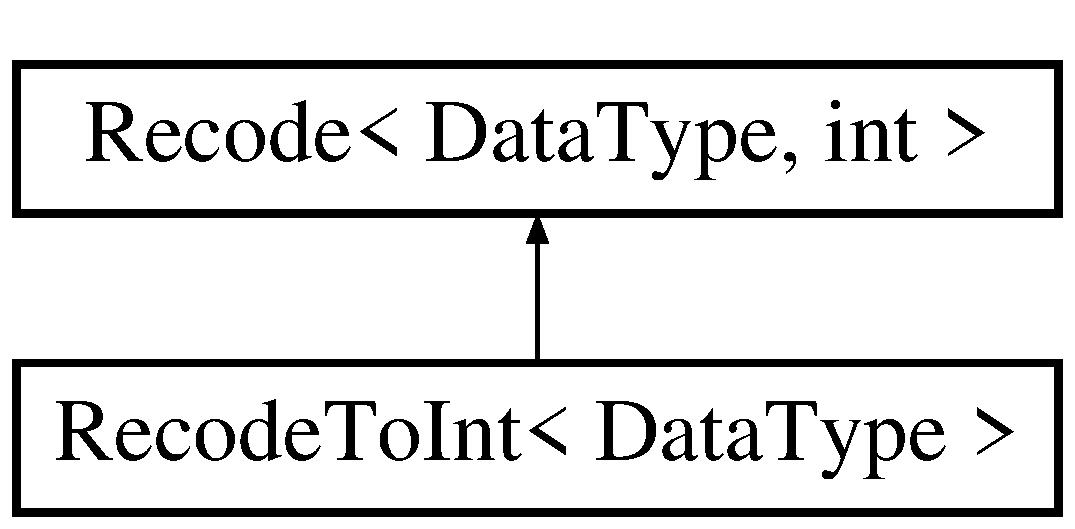
\includegraphics[height=2cm]{class_recode_to_int}
\end{center}
\end{figure}
\subsection*{Public Member Functions}
\begin{CompactItemize}
\item 
{\bf Recode\-To\-Int} ()\label{class_recode_to_int_7afccf5cc723177c720d62d7eedc5414}

\begin{CompactList}\small\item\em Contructor. \item\end{CompactList}\item 
template$<$class Container$>$ {\bf Recode\-To\-Int} (Container \&itemset)
\begin{CompactList}\small\item\em Contructor used to construct the recode object initialized with a SET (not a multi set) of Data\-Type. \item\end{CompactList}\item 
virtual {\bf $\sim$Recode\-To\-Int} ()\label{class_recode_to_int_264d862332a6695baeeb1625d22b8434}

\begin{CompactList}\small\item\em Destructor. \item\end{CompactList}\item 
{\bf Recode\-To\-Int} (const {\bf Recode\-To\-Int} \&rec)\label{class_recode_to_int_8ae90856c152323463a232005e5fb878}

\begin{CompactList}\small\item\em Copy contructor. \item\end{CompactList}\item 
{\bf Recode\-To\-Int} \& {\bf operator=} (const {\bf Recode\-To\-Int} \&rec)\label{class_recode_to_int_40bf1ee6b8a5e79af7a688b3b59eb009}

\begin{CompactList}\small\item\em Affectation operator. \item\end{CompactList}\item 
template$<$class Container$>$ vector$<$ int $>$ \& {\bf operator()} (Container \&itemset)
\begin{CompactList}\small\item\em Map elements of the input data in internals ids. \item\end{CompactList}\item 
template$<$class Input\-Iterator$>$ vector$<$ int $>$ \& {\bf operator()} (Input\-Iterator first, Input\-Iterator last)
\begin{CompactList}\small\item\em Map elements of the input data in internals ids. \item\end{CompactList}\item 
virtual int {\bf operator()} (Data\-Type item)
\begin{CompactList}\small\item\em Map an element of the input data in an internals id. \item\end{CompactList}\item 
template$<$class Container$>$ vector$<$ Data\-Type $>$ \& {\bf remap} (Container \&itemset)
\begin{CompactList}\small\item\em Remap internals ids in elements of the input data . \item\end{CompactList}\item 
void {\bf remap} (vector$<$ int $>$ $\ast$itemset, vector$<$ Data\-Type $>$ $\ast$remap\-Itemsets)
\begin{CompactList}\small\item\em Remap internals set of ids in the corresponfing set of elements of the input data . \item\end{CompactList}\item 
template$<$class Input\-Iterator$>$ vector$<$ Data\-Type $>$ \& {\bf remap} (Input\-Iterator first, Input\-Iterator last)
\begin{CompactList}\small\item\em Remap internals ids in elements of the input data . \item\end{CompactList}\item 
virtual Data\-Type {\bf remap} (int item)
\begin{CompactList}\small\item\em Map an element of the input data in an internals id. \item\end{CompactList}\end{CompactItemize}
\subsection*{Public Attributes}
\begin{CompactItemize}
\item 
vector$<$ Data\-Type $>$ {\bf int\-Id\-Toid}\label{class_recode_to_int_0286413c937d57bc153465e4c7625d6c}

\begin{CompactList}\small\item\em vector used to map the internal id to the real elemnt. \item\end{CompactList}\end{CompactItemize}


\subsection{Detailed Description}
\subsubsection*{template$<$class Data\-Type$>$ class Recode\-To\-Int$<$ Data\-Type $>$}

Class {\bf Recode\-To\-Int}{\rm (p.\,\pageref{class_recode_to_int})} recode data oftype T in integers and stor the mapping. 

The template parameter is the original type of the elements to recode in int. The internal id of the element are defined wrt the order they are passed to the functor. For example the first element passed to the functor have the id 0, the second element 1,... 



\subsection{Constructor \& Destructor Documentation}
\index{RecodeToInt@{Recode\-To\-Int}!RecodeToInt@{RecodeToInt}}
\index{RecodeToInt@{RecodeToInt}!RecodeToInt@{Recode\-To\-Int}}
\subsubsection{\setlength{\rightskip}{0pt plus 5cm}template$<$class Data\-Type$>$ template$<$class Container$>$ {\bf Recode\-To\-Int}$<$ Data\-Type $>$::{\bf Recode\-To\-Int} (Container \& {\em itemset})\hspace{0.3cm}{\tt  [inline]}}\label{class_recode_to_int_c79659f9e5d7b2a894cb9edaed32b32d}


Contructor used to construct the recode object initialized with a SET (not a multi set) of Data\-Type. 

Since recode is empty, the sets are new sets to recode, there is no need to search if they already recoded. 

\subsection{Member Function Documentation}
\index{RecodeToInt@{Recode\-To\-Int}!operator()@{operator()}}
\index{operator()@{operator()}!RecodeToInt@{Recode\-To\-Int}}
\subsubsection{\setlength{\rightskip}{0pt plus 5cm}template$<$class Data\-Type$>$ int {\bf Recode\-To\-Int}$<$ Data\-Type $>$::operator() (Data\-Type {\em item})\hspace{0.3cm}{\tt  [virtual]}}\label{class_recode_to_int_84e738bd2a7faf92a7d916e995689cab}


Map an element of the input data in an internals id. 

\begin{Desc}
\item[Returns:]the new id. \end{Desc}


Implements {\bf Recode$<$ Data\-Type, int $>$} {\rm (p.\,\pageref{class_recode_266e8a09b4576e02aab3cd6590a9ffbf})}.\index{RecodeToInt@{Recode\-To\-Int}!operator()@{operator()}}
\index{operator()@{operator()}!RecodeToInt@{Recode\-To\-Int}}
\subsubsection{\setlength{\rightskip}{0pt plus 5cm}template$<$class Data\-Type$>$ template$<$class Input\-Iterator$>$ vector$<$ int $>$ \& {\bf Recode\-To\-Int}$<$ Data\-Type $>$::operator() (Input\-Iterator {\em first}, Input\-Iterator {\em last})}\label{class_recode_to_int_51f3193e2ace542f3041ee0f3dca8deb}


Map elements of the input data in internals ids. 

\begin{Desc}
\item[Parameters:]
\begin{description}
\item[{\em first}]iterator on the first element \item[{\em last}]iterator on the element after the last \end{description}
\end{Desc}
\begin{Desc}
\item[Returns:]the new ids. \end{Desc}
\index{RecodeToInt@{Recode\-To\-Int}!operator()@{operator()}}
\index{operator()@{operator()}!RecodeToInt@{Recode\-To\-Int}}
\subsubsection{\setlength{\rightskip}{0pt plus 5cm}template$<$class Data\-Type$>$ template$<$class Container$>$ vector$<$ int $>$ \& {\bf Recode\-To\-Int}$<$ Data\-Type $>$::operator() (Container \& {\em itemset})}\label{class_recode_to_int_7d3d3ea423abd8e055ba4483744fba04}


Map elements of the input data in internals ids. 

\begin{Desc}
\item[Parameters:]
\begin{description}
\item[{\em itemset}]set of elements to recode in int. \end{description}
\end{Desc}
\begin{Desc}
\item[Returns:]the new ids. \end{Desc}


Reimplemented from {\bf Recode$<$ Data\-Type, int $>$} {\rm (p.\,\pageref{class_recode_d4fc62868c9f2097c762a6e0c66ae685})}.\index{RecodeToInt@{Recode\-To\-Int}!remap@{remap}}
\index{remap@{remap}!RecodeToInt@{Recode\-To\-Int}}
\subsubsection{\setlength{\rightskip}{0pt plus 5cm}template$<$class Data\-Type$>$ virtual Data\-Type {\bf Recode\-To\-Int}$<$ Data\-Type $>$::remap (int {\em item})\hspace{0.3cm}{\tt  [inline, virtual]}}\label{class_recode_to_int_338aeadf35cd3aad00d61d313bdf59d2}


Map an element of the input data in an internals id. 

\begin{Desc}
\item[Returns:]the new id. \end{Desc}
\index{RecodeToInt@{Recode\-To\-Int}!remap@{remap}}
\index{remap@{remap}!RecodeToInt@{Recode\-To\-Int}}
\subsubsection{\setlength{\rightskip}{0pt plus 5cm}template$<$class Data\-Type$>$ template$<$class Input\-Iterator$>$ vector$<$Data\-Type$>$\& {\bf Recode\-To\-Int}$<$ Data\-Type $>$::remap (Input\-Iterator {\em first}, Input\-Iterator {\em last})\hspace{0.3cm}{\tt  [inline]}}\label{class_recode_to_int_a138eafdc7693c0cf5057c6fc786d80b}


Remap internals ids in elements of the input data . 

\begin{Desc}
\item[Parameters:]
\begin{description}
\item[{\em first}]iterator on the first element to remap. \item[{\em last}]iterator on the element after the last to remap. \end{description}
\end{Desc}
\begin{Desc}
\item[Returns:]the original ids. \end{Desc}
\index{RecodeToInt@{Recode\-To\-Int}!remap@{remap}}
\index{remap@{remap}!RecodeToInt@{Recode\-To\-Int}}
\subsubsection{\setlength{\rightskip}{0pt plus 5cm}template$<$class Data\-Type$>$ void {\bf Recode\-To\-Int}$<$ Data\-Type $>$::remap (vector$<$ int $>$ $\ast$ {\em itemset}, vector$<$ Data\-Type $>$ $\ast$ {\em remap\-Itemsets})\hspace{0.3cm}{\tt  [inline]}}\label{class_recode_to_int_8dcffed515a66b6a64c837933dca615e}


Remap internals set of ids in the corresponfing set of elements of the input data . 

\begin{Desc}
\item[Parameters:]
\begin{description}
\item[{\em itemset}]set of elements to recode in input Data type. \item[{\em remap\-Itemsets}]for the original ids . \end{description}
\end{Desc}
\index{RecodeToInt@{Recode\-To\-Int}!remap@{remap}}
\index{remap@{remap}!RecodeToInt@{Recode\-To\-Int}}
\subsubsection{\setlength{\rightskip}{0pt plus 5cm}template$<$class Data\-Type$>$ template$<$class Container$>$ vector$<$Data\-Type$>$\& {\bf Recode\-To\-Int}$<$ Data\-Type $>$::remap (Container \& {\em itemset})\hspace{0.3cm}{\tt  [inline]}}\label{class_recode_to_int_814de08675679f300ae7171f560b0e61}


Remap internals ids in elements of the input data . 

\begin{Desc}
\item[Parameters:]
\begin{description}
\item[{\em itemset}]set of elements to recode in input Data type. \end{description}
\end{Desc}
\begin{Desc}
\item[Returns:]the original ids . \end{Desc}


The documentation for this class was generated from the following file:\begin{CompactItemize}
\item 
F:/i\-Zi/util/Recode\-To\-Int.hxx\end{CompactItemize}
